
%(BEGIN_QUESTION)
% Copyright 2008, Tony R. Kuphaldt, released under the Creative Commons Attribution License (v 1.0)
% This means you may do almost anything with this work of mine, so long as you give me proper credit

The Rockwell/Allen-Bradley MicroLogix 1000 programmable logic controller (PLC) can handle up to four analog input signals: two with a 0-10 V maximum range and two with a 0-20 mA maximum signal range.  This PLC's analog input terminal block looks like this (the internal resistors are shown inside the PLC box):

$$\includegraphics[width=15.5cm]{i03252x01.eps}$$

Sketch the appropriate wiring to connect a pair of 4-20 mA loop-powered transmitters to the two current inputs (IA/2 and IA/3) on the PLC.

\vfil 

Note: the two ``IA SHD'' terminals are provided for cable shield conductor attachment.  You may ignore cable shield wires and these terminals for simplicity's sake.

\underbar{file i03252}
\eject
%(END_QUESTION)





%(BEGIN_ANSWER)

This is a graded question -- no answers or hints given!
 
%(END_ANSWER)





%(BEGIN_NOTES)

Since we are using the current (low-resistance) analog channels on this PLC, we need to connect each PLC input in {\it series} with its respective 4-20 mA transmitter, since we know that only in a series circuit is current guaranteed to be the same through all components at any given time.

\vskip 10pt

This is just one possible solution:

$$\includegraphics[width=15.5cm]{i03252x02.eps}$$

A helpful problem-solving technique for any DC circuit-sketching problem is to label voltage polarities and current directions for each component in the circuit based on its status as either an electrical {\it source} or an electrical {\it load}.  Sources have conventional flow current exiting the positive terminal, while loads have conventional flow current entering the positive terminal.

%INDEX% Pictorial circuit review (4-20 mA loop)

%(END_NOTES)


